\documentclass{article}
\usepackage{hyperref}
\usepackage{graphicx}
\usepackage{geometry}

 \geometry{
 a4paper,
 left=20mm,
 right=20mm,
 top=20mm,
 }
 
\hypersetup{
    colorlinks,
    citecolor=black,
    filecolor=black,
    linkcolor=black,
    urlcolor=black
}

\begin{document}
    
    \section{Notification Subsystem}
    
    \subsection{Overview}
    The notifications module provides notifications to system users regarding
    particular system updates that a user would like to be notified about through
    some medium external to the application.
    
    \subsection{External Interface Requirements}
    
    \subsubsection{User Interfaces}
    
    The subsystem will allow for notifications to be pushed to registered users in the form of E-mails. The E-mails will have a descriptive subject associated with it and will be accessible from any device that allows a form of e-mail service.

    \begin{flushleft}
    

    The subsystem will allow for notifications to be pushed to registered users in the form of SMS's. the SMS's will only have a senders name which will indicate the type of notification and the SMS's content will then go on to expand on the notifications description.
	\newline

    The subsystem will interact with users mostly on a cellular device and a colour screen will be required to get the most out of the application in terms of the E-mail service, SMS's on the other hand are a vital part of most cellular devices and in most cases no extra functionality is required.

   	  \end{flushleft}
   	\subsubsection{Hardware Interfaces}
    \begin{flushleft}
    With the use of most cellular devices, a colour screen will be required for the use of e-mails and the device must in all cases be able to display information in a way that is understandable by the user.
\newline

    The device must have the appropriate hardware in place to allow a form of data connection between itself and the internet.
    \end{flushleft}
	
	\subsubsection{Software Interfaces}
	\begin{flushleft}
	The application will require an e-mail and SMS application in order to receive notifications of this type.
\newline

	The subsystem will need to have access to a database of users such that they can be added to the user lists for the particular type of notification/s of their preference. These lists will then be referenced when the notifications are being sent to the users.
\end{flushleft}	    

	\subsubsection{Communication Interfaces}
	\begin{flushleft}
	The subsystem will need to communicate with any other subsystem that wishes to create and send out notifications to the users.
\newline

	The subsystem will need to communicate with an automated E-Mail service to send out the mass e-mails to the users.
\newline

	The subsystem will need to communicate with an automated SMS service to send out the mass SMS's to the users.
\newline

	The users will need to have the appropriate communications interfaces available to allow them to receive notifications. This would include a working cellphone SIM card with a registered cellphone number and/or a working e-mail account that is accessible on a device with a data connection of some form.
	\end{flushleft}
	
	\subsection{Performance Requirements}
    \begin{flushleft}
    The notifications will have to be pushed out in a timely manner such that the time between creation and time of sending of notifications is minimal.
    \newline
    
    The system will also have to handle sending bulk e-mails and SMS's from multiple notifying modules in a manner that will not cripple the system or put the system at risk.
    \end{flushleft}
    
    \subsection{Design Constraints}
    \begin{flushleft}
    Notifications should not be long such that loading times are affected(e-mail) or that partitioning of messages occurs(sms)
    \newline
    Notifications should be pushed out within a given time frame.
    \newline
    Notifications should conform to the rules of the medium of transport.
    \newline
    No unnecessary data/information should be sent in these notifications. 
    \end{flushleft}
    
    
    \clearpage
    \subsubsection{UML Diagrams}
    
    \begin{figure}[h!]
        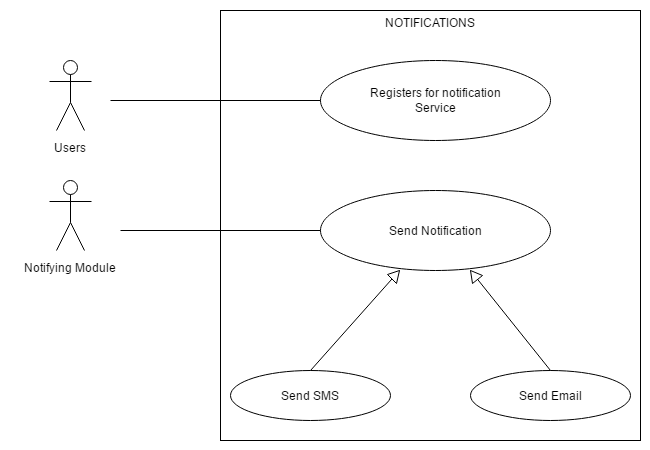
\includegraphics[width=\textwidth]{Notifications_Use_Case.png}
    \end{figure}
    Notification Use Case Diagram
    
    \mbox{}\\
    \bigskip
    \clearpage
    
    \begin{figure}[h!]
      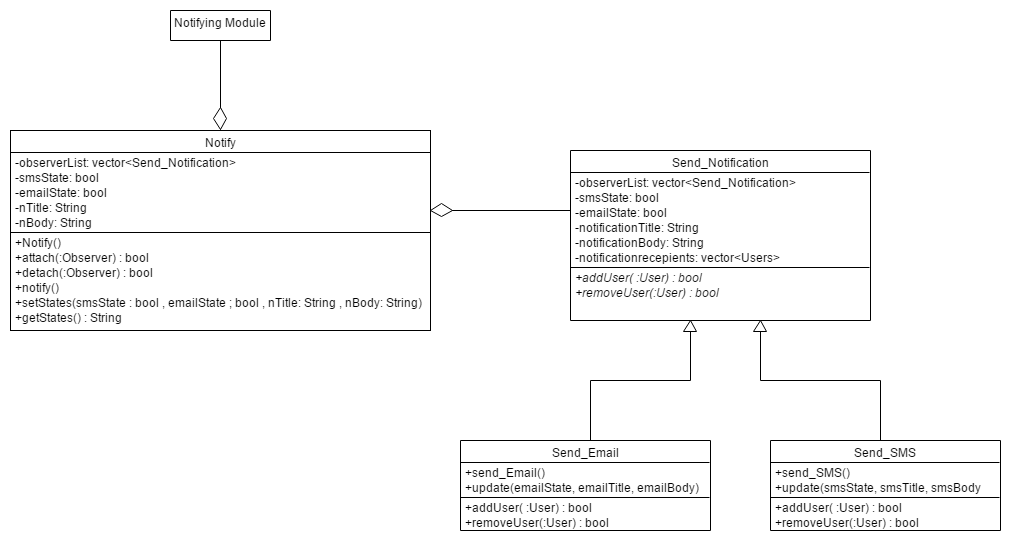
\includegraphics[width=\textwidth]{Notifications_Class_Diagram.png}
    \end{figure}
    Notification Class Diagram
    
    \begin{flushleft}
    
        For the notifications subsystem the observer design pattern came to light, as this pattern allows objects to change state and all of its dependents follow suit. This allows a notification state to be used that can update whether or not a notification needs to be sent out. In this case the push method of observer was used. Also evident is the template design pattern that uses the concrete observers to redefine the way in which the notifications are sent. Notifying modules are also given the flexibility to decide which medium/s are used for the notification.
        
        \bigskip

        
        There are methods in the Send Email and Send SMS classes that allow users to be added to the user lists for the notifications to either or both of these mediums. There is also provision for more notification mediums to be added in the future and these can be attached to the Notify class. Should a notification medium be unavailable it can be detached from the Notify class until it is available. The Notify class can be called from any other module that would like to request a notification to be sent out to users which allows for modularity.
        
        \bigskip

        Notify: Subject
        

        Send Notification: Observer(Observer) / Abstract Method(Template)
        

        Send Email: Concrete Observer1(Observer) /Concrete Method(Template)
        

        Send SMS: Concrete Observer2(Observer) / Concrete Method(Template)
    
    \end{flushleft}
    
    \mbox{}\\
    \bigskip
    \clearpage
    
    \begin{figure}[h!]
        \includegraphics[width=\textwidth]{Notification_Sequence_Diagram.png}
    \end{figure}
    Notification Sequence Diagram
    
    \mbox{}\\
    \bigskip
    \clearpage
    
    \begin{figure}[h!]
        \includegraphics[width=\textwidth]{User_Register_Notification.png}
    \end{figure}
    Add User Activity Diagram
    
    \mbox{}\\
    \bigskip
    \clearpage
    
    \begin{figure}[h!]
        \includegraphics[width=\textwidth]{Notifications_Activity_Diagram.png}
    \end{figure}
    Send Notification Activity Diagram
    
    \mbox{}\\
    \bigskip
    \clearpage
    
    \begin{figure}[h!]
        \begin{center}
            \includegraphics[width=0.6\textwidth]{Notification_State_Diagram.png}
        \end{center}
    \end{figure}
    Notification State Diagram
    
    \mbox{}\\
\end{document}
